\documentclass[12pt, oneside]{article}
\usepackage{geometry}                		% See geometry.pdf to learn the layout options. There are lots.
\geometry{letterpaper} 
\usepackage{amsmath}
\usepackage{amsthm}
\usepackage{amssymb}
\usepackage{graphicx}
\usepackage{color}
\usepackage{float}
\usepackage{subfig}
\usepackage[flushleft]{threeparttable}
\usepackage{gensymb}
\usepackage{multirow}
\usepackage[dvipsnames]{xcolor}
\newcommand{\BibTeX}{\textsc{Bib}\TeX}

\title{P3D2HDF5}


\begin{document}
\maketitle

\section{Using the Tool}
p3d2HDF5 is a tool that allows you to convert between the file types plot3d and HDF5, additionally it allows for the separation of large data files
into smaller ones using several different parameters.

Some general notes:

The variables i,j,k max should be set to the dimensions of your data set, while the file paths should be a valid path to your data set from where the code is being run.

\subsection{Separating using kioplane}
In order to use this function set the convert flow/grid tag to 1 and choose the format 3. Separating using kioplane will divide the data set into planes with a k dimension equal 
to kioplane and any remaining data into one last data set.

\begin{figure}[H]
\centering
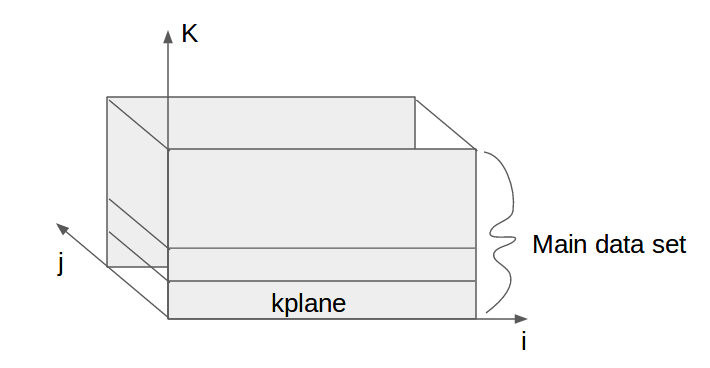
\includegraphics[width=0.5\textwidth]{FIGS/Kplane.png}

\caption{{\footnotesize Example of Kplane Cut}}
\label{fig: } 
\end{figure}

\subsection{Separating using inode}
In order to use this function set the convert flow/grid tag to 1 and choose format 4. Separating using inode will divide the data set into an inode amount of 
as evenly spaced as possible data sets cut along the i direction, this can be used, if inode is set to the amount of nodes used, 
to divide the data space up into sections that a single node would have handled during calculations.

\begin{figure}[H]
\centering
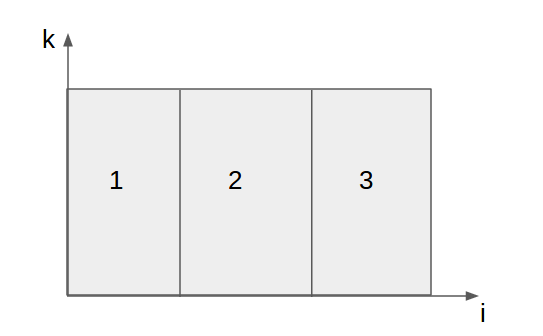
\includegraphics[width=0.5\textwidth]{FIGS/Inode.png}

\caption{{\footnotesize example with inode=3}}
\label{fig: } 
\end{figure}

\subsection{Separating using jnode}
This feature is only available in the parallel version of the code and is used by setting the format to 5. This will behave exactly like using inode except it will divide
data sets in the j direction.

\subsection{General notes for using the parallel version}
The parallel version of the code makes use of multiple processors in order to speed up the code when accessing very large data sets. This version of the code is located
in the parallel folder. In order to run it check the processor amount requirements located in the input file and make use of the mpirun command

\begin{verbatim}
 mpirun -np numberofprocessors p3dh5 < p3dh5.inp 
\end{verbatim}



\end{document}
